\documentclass{article}
\usepackage[utf8]{inputenc}
\usepackage[a4paper,left=3.5cm,right=3.5cm,top=2cm,bottom=2cm]{geometry}
\usepackage{crop,graphicx,amsmath,array,color,amssymb,fancyhdr,lineno}
\usepackage{flushend,stfloats,amsthm,chngpage,times,,lipsum,lastpage} 
\usepackage{calc,listings,color,wrapfig,tabularx,longtable,enumitem}
\usepackage{multirow}
\usepackage{caption}
\usepackage{subcaption}
\usepackage{xcolor}
\usepackage{tcolorbox}
\definecolor{shadecolor}{rgb}{0.86,0.86,0.86}
\usepackage{float}
\usepackage{lineno}
\usepackage{csquotes}
\usepackage[italian]{babel}
\usepackage[hidelinks]{hyperref}
\usepackage{fancyhdr}
\usepackage{booktabs}

\title{Confronto tra Algoritmi di String Matching}
\author{Eros Pinzani}

\fancyhf{}
\fancyhead[L]{Pinzani Eros}
\fancyhead[R]{Laboratorio di Algoritmi e Strutture Dati}
\fancyfoot[C]{\thepage}
\renewcommand{\headrulewidth}{0.4pt}

\lstset{
  literate={!=}{{$\neq$}}1 {pi}{{$\pi$}}1,
  basicstyle=\ttfamily
}

\begin{document}
\pagestyle{fancy}

\begin{titlepage}
    \centering
    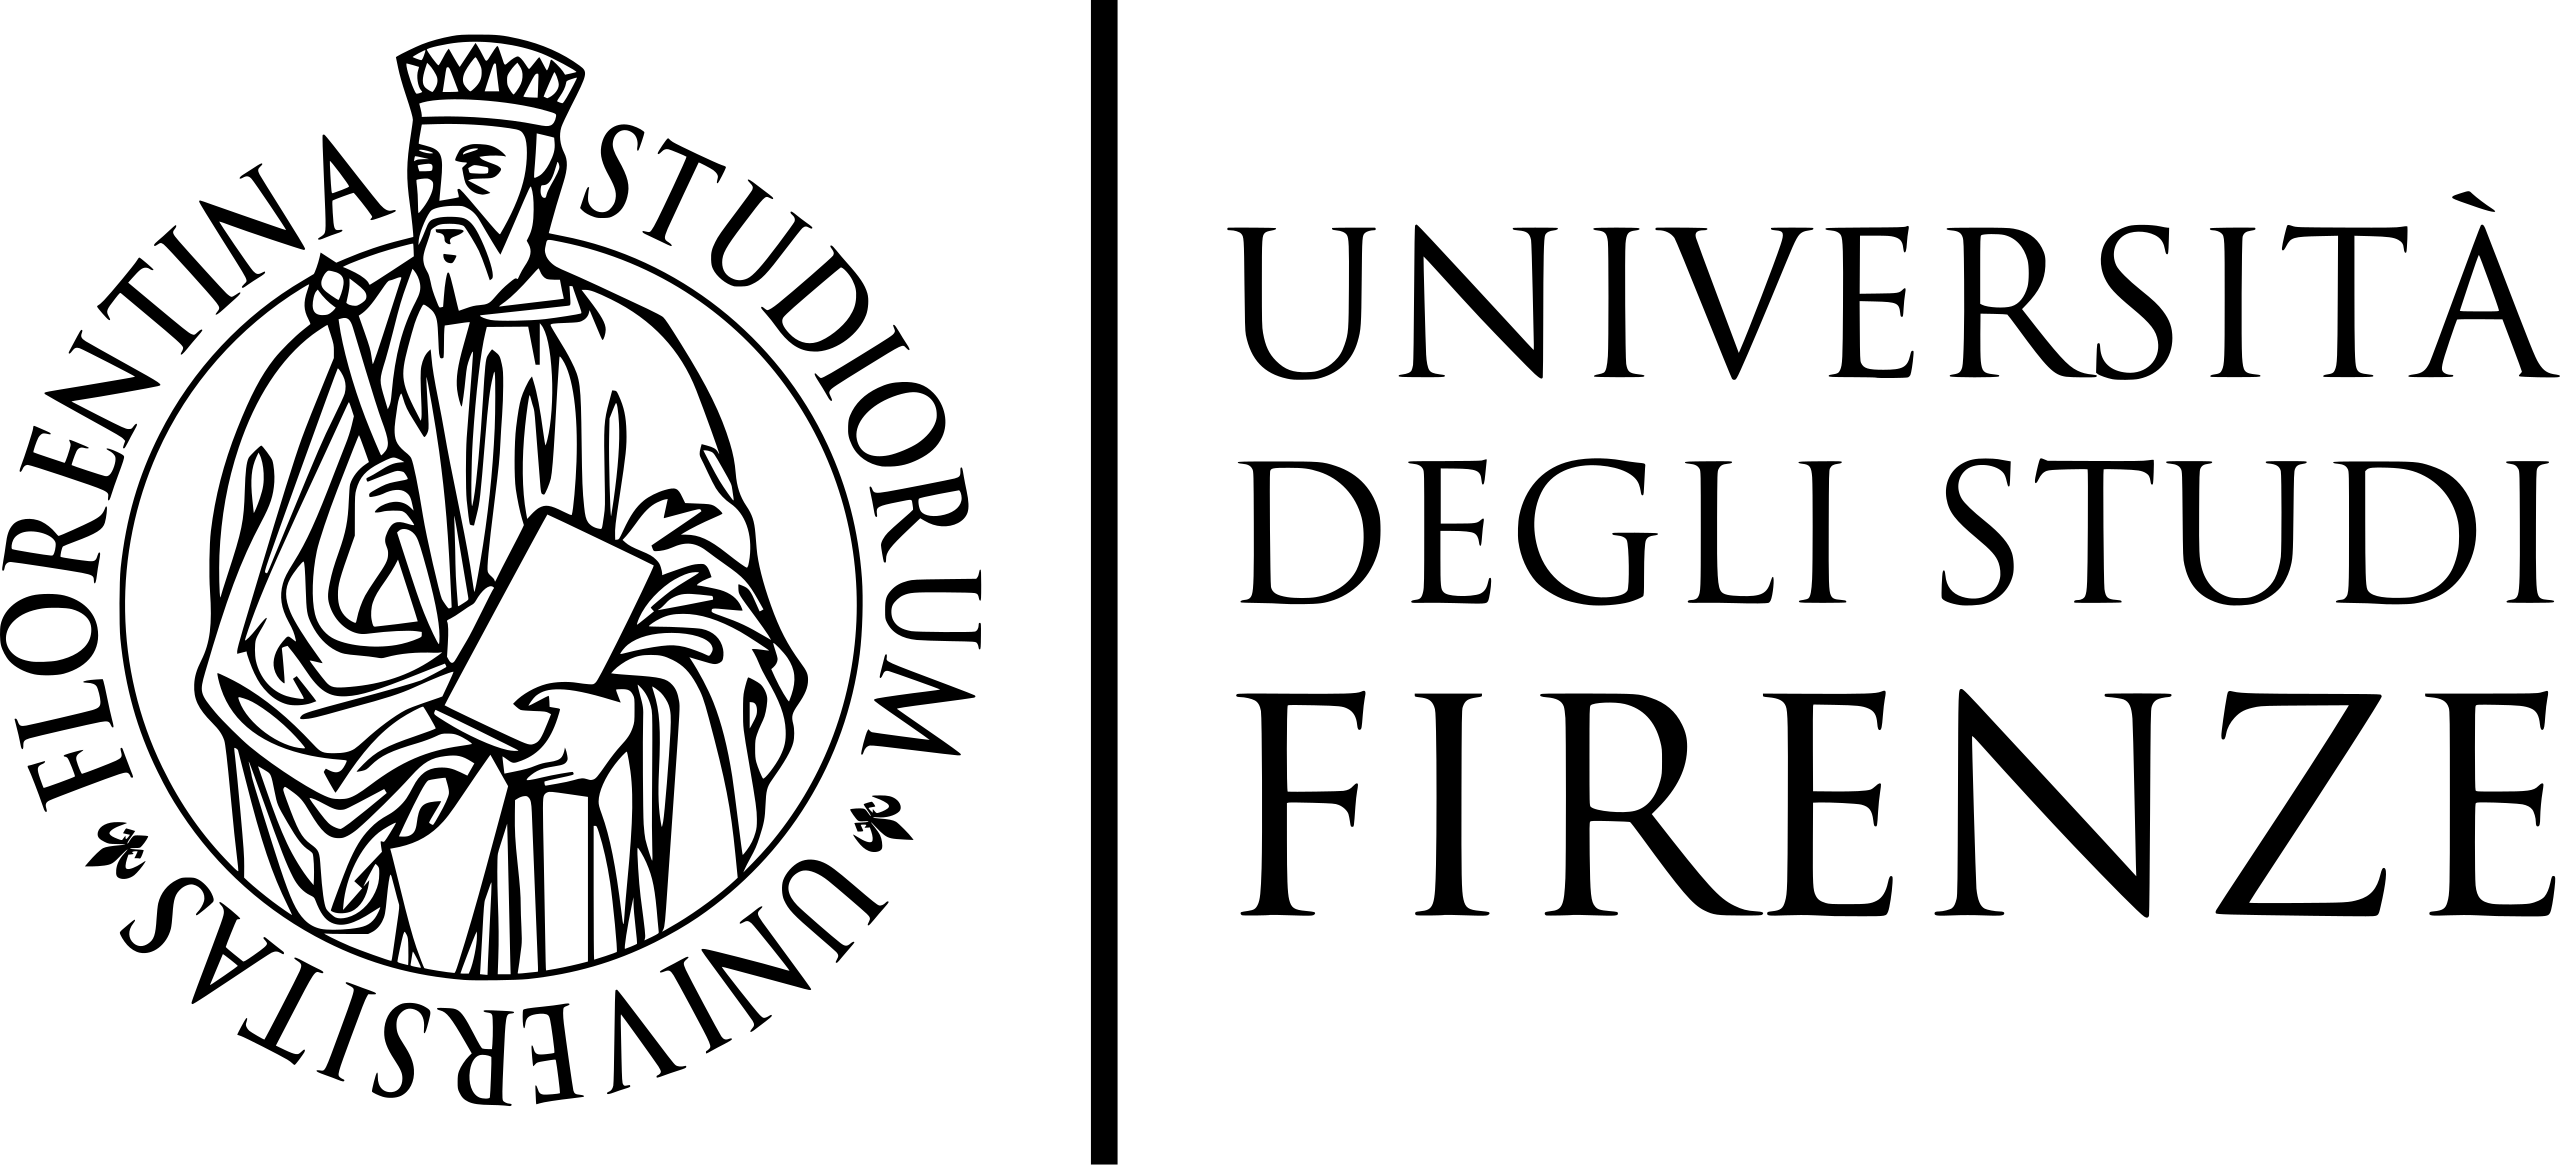
\includegraphics[width=0.90\textwidth]{img/Logo_universita_firenze.svg.png}\par\vspace{1cm}
    {\scshape\LARGE Università degli Studi di Firenze \par}
    \vspace{0.25cm}
    {\scshape\Large Dipartimento di Ingegneria dell'Informazione\par}
    \vspace{0.5cm}
    \rule{\linewidth}{0.4pt}
    \begin{center}
        {\Huge{\bfseries \textbf{Confronto tra Algoritmi di String Matching}\par}}
    \end{center}
    \rule{\linewidth}{0.4pt}
    \vspace{1cm}

    \begin{minipage}[t]{0.4\textwidth}
        \begin{flushleft} \large
            \emph{Autore:}\par
            Eros Pinzani\par
        \end{flushleft}

        \begin{flushleft} \large
            \emph{N° Matricola:}\par
            7030989\par
        \end{flushleft}
    \end{minipage}
    \hfill
    \begin{minipage}[t]{0.4\textwidth}
        \begin{flushleft} \large\raggedleft
            \emph{Corso:}\par
            Algoritmi e Strutture Dati
        \end{flushleft}

        \begin{flushleft} \large\raggedleft
            \emph{Docente corso:}\par
            Simone Marinai\par
        \end{flushleft}
    \end{minipage}

\end{titlepage}

\newpage
\renewcommand{\contentsname}{Indice}
\tableofcontents
\addcontentsline{toc}{section}{Elenco delle figure}
\listoffigures
\pagenumbering{arabic}

\newpage
\section{Introduzione generale}
\subsection{Breve descrizione dello svolgimento degli esercizi}
Per ogni esercizio suddividiamo la sua descrizione in 4 parti fondamentali:

\begin{itemize}
    \item \textbf{Spiegazione teorica del problema}: qui è dove si descrive il problema che andremo ad affrontare in modo teorico partendo dagli assunti del libro di Algoritmi e Strutture Dati e da altre fonti.
    \item \textbf{Documentazione del codice}: in questa parte spieghiamo come il codice dell'esercizio viene implementato.
    \item \textbf{Descrizione degli esperimenti condotti}: partendo dal codice ed effettuando misurazioni varie cerchiamo di verificare le ipotesi teoriche.
    \item \textbf{Analisi dei risultati sperimentali}: dopo aver svolto i vari esperimenti riflettiamo sui vari risultati ed esponiamo una tesi.
\end{itemize}

\subsection{Specifiche della piattaforma di test}
La piattaforma di test sarà la stessa per ogni esercizio che vedremo. Partiamo dall'hardware del computer fondamentale da conoscere per questo esercizio:

\begin{itemize}
    \item \textbf{CPU} : AMD Ryzen™ 5 PRO 7540U (da 3,2 GHz fino a 4,9 GHz)
    \item \textbf{RAM} : 16 GB LPDDR5X-6.400MT/s
    \item \textbf{SSD} : 512 GB M.2 2280 PCIe Gen4 TLC Opal
\end{itemize}

\noindent Il linguaggio di programmazione utilizzato sarà Python e la piattaforma in cui il codice è stato scritto e 'girato' è l'IDE \textbf{Visual Studio Code}. La stesura di questo testo è avvenuta tramite l'utilizzo di \textbf{Visual Studio Code} e opportune estensioni.

\newpage

\part{Algoritmo ``ingenuo'' vs Algoritmo KMP}

\begin{tcolorbox}[colback=lightgray!20,
        colframe=black,
        arc=3mm, auto outer arc,]

    \textbf{Esercizio A}
    \begin{itemize}
        \item Vogliamo confrontare gli algoritmi ``ingenuo'' e KMP per effettuare string matching
        \item Per fare questo dovremo:
              \begin{itemize}
                  \item Scrivere i programmi Python che:
                        \begin{itemize}
                            \item implementino quanto richiesto
                            \item eseguono un insieme di test che ci permettano di comprendere vantaggi e svantaggi delle diverse implementazioni
                        \end{itemize}
                  \item Svolgere ed analizzare opportuni esperimenti
                  \item Scrivere una relazione che descriva quanto fatto
              \end{itemize}
    \end{itemize}
\end{tcolorbox}

\section{Spiegazione teorica del problema }

\subsection{Introduzione}
Nella seguente parte della relazione viene descritta l'implementazione degli algoritmi di string matching ``\textbf{ingenuo}'' e \textbf{Knuth-Morris-Pratt}, d'ora in poi chiamato \textbf{KMP} per semplicità. Questi algoritmi permettono di ricercare una data stringa, chiamata \textbf{pattern}, all'interno di un \textbf{testo} più o meno complesso. Verranno quindi messi a confronto i due algoritmi per valutarne la complessità in termini di tempo necessario e numero di confronti effettuati prima di trovare tutte quante le occorrenze.

\subsection{Cos'è un algoritmo di string matching?}
Gli algoritmi di string matching sono algoritmi che permettono di trovare una o più occorrenze di una stringa, chiamata \textbf{pattern}, all'interno di un'altra stringa, chiamata \textbf{testo}. Questi algoritmi sono utilizzati in molti campi, ad esempio nella ricerca di pattern in sequenze di DNA oppure vengono utilizzati da motori di ricerca per individuare pagine web pertinenti alle query.
Andiamo ora ad analizzare nel dettaglio gli algoritmi ``\textbf{ingenuo}'' e \textbf{KMP} osservando che a parità di occorrenze del pattern trovate il secondo algoritmo risulta essere più efficiente del primo.

\subsubsection{Algoritmo ``ingenuo''}
L'algoritmo ``\textbf{ingenuo}'' è il più semplice da implementare e consiste nel confrontare il pattern con ogni sottostringa del testo di lunghezza uguale al pattern. In questo modo, l'algoritmo scorre il testo e per ogni posizione confronta il pattern con la sottostringa del testo. Se i caratteri corrispondono, l'algoritmo continua a confrontare i caratteri successivi fino a quando non trova una occorrenza completa o un carattere diverso. In caso di occorrenza completa, l'algoritmo registra la posizione in cui è stata trovata l'occorrenza.
\begin{itemize}
    \item Pseudocodice:
          \begin{figure}[H]
              \centering
              \begin{lstlisting}
            NAIVE-STRING-MATCHER(T, P)
                n = T.length
                m = P.length
                for s = 0 to n - m
                    if P[1...m] == T[s + 1...s + m]
                        stampa "Occorrenza del pattern con
                        spostamento s"
            \end{lstlisting}
              \caption{Pseudocodice dell'algoritmo ``ingenuo''}
              \label{fig:naive-pseudocode}
          \end{figure}
    \vspace{0.5cm}
    \item Descrizione dell'algoritmo:
          \begin{enumerate}
              \item L'algoritmo inizia salvando le lunghezze del testo e del pattern nelle rispettive variabili \textit{n} e \textit{m}.
              \item Successivamente, inizia un ciclo che scorre il testo da 0 a \textit{n} - \textit{m}
              \item Quindi confronta tutto il pattern con la sottostringa del testo di lunghezza \textit{m} a partire dalla posizione \textit{s}.
              \item Se la condizione viene rispettata allora viene stampata la posizione \textit{s} in cui è stata trovata l'occorrenza.
          \end{enumerate}
    \item Implementazione:
          \begin{figure}[H]
              \centering
              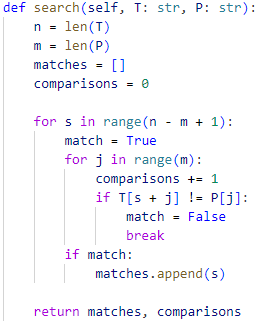
\includegraphics[width=0.3\textwidth]{img/Naive_search.png}
              \caption{Implementazione Python dell'algoritmo ``ingenuo''}
              \label{fig:naive-implementation}
          \end{figure}
    \item Motivazioni per l'uso dell'algoritmo ``ingenuo'':
          \begin{itemize}
              \item Semplicità di implementazione
              \item Efficace per casi semplici e non ripetitivi
              \item Nessuna pre-elaborazione del pattern
          \end{itemize}
\end{itemize}

\subsubsection{Algoritmo KMP}
L'algoritmo \textbf{KMP} è un algoritmo più avanzato rispetto a quello ``\textbf{ingenuo}'' perché evita confronti ridondanti. Inizialmente viene analizzato il pattern e l'algoritmo costruisce una struttura ausiliaria chiamata \textbf{funzione prefisso $\pi$} grazie alla quale, durante la fase di ricerca, in caso di discordanza tra pattern e testo, permette di saltare alcuni confronti inutili.\\
La funzione prefisso $\pi$ associa ad ogni posizione \textit{i} del pattern il numero massimo di caratteri iniziali (prefisso) che coincidono con un suffisso della sottostringa del pattern P[1...\textit{i}]. Ovvero, $\pi[i]$ rappresenta la lunghezza del più lungo prefisso del pattern che è anche un suffisso di P[1...\textit{i}]. È grazie a questa funzione che l'algoritmo stabilisce di quanto può essere traslato in avanti il pattern, continuando a mantenere allineati i caratteri già confrontati.
\begin{itemize}
    \item Pseudocodice:
          \begin{figure}[H]
              \begin{lstlisting}
            COMPUTE-PREFIX-FUNCTION(P)
                m = P.length
                Sia pi[1...m] un nuovo array
                pi[1] = 0
                k = 0
                for q = 2 to m
                    while k > 0 and P[k + 1] != P[q]
                        k = pi[k]
                    if P[k + 1] == P[q]
                        k = k + 1
                    pi[q] = k
                return pi
            \end{lstlisting}
              \caption{Pseudocodice della funzione dei prefissi}
              \label{fig:prefix-function-pseudocode}
          \end{figure}
          \begin{figure}[H]
              \centering
              \begin{lstlisting}
            KMP-MATCHER(T, P)
                n = T.length
                m = P.length
                pi = COMPUTE-PREFIX-FUNCTION(P)
                q = 0
                for i = 1 to n
                    while q > 0 and P[q + 1] != T[i]
                        q = pi[q]
                    if P[q + 1] == T[i]
                        q = q + 1
                    if q == m
                        stampa "Occorrenza del pattern con
                        spostamento i - m"
                        q = pi[q]
            \end{lstlisting}
              \caption{Pseudocodice dell'algoritmo KMP}
              \label{fig:KMP-pseudocode}
          \end{figure}
    \item Descrizione dell'algoritmo:
          \begin{enumerate}[label=\arabic*a.]
              \item La funzione \textbf{COMPUTE-PREFIX-FUNCTION} inizia con il salvare la lunghezza del pattern nella variabile \textit{m}.
              \item Viene poi creato un array $\pi$ di lunghezza \textit{m}. Ogni elemento di questo array rappresenta la lunghezza del più lungo prefisso del pattern che è anche un suffisso della sottostringa del pattern P[1...\textit{q}].
              \item Viene poi inizializzato il primo elemento dell'array $\pi$ a 0.
              \item Quindi viene inizializzata la variabile \textit{k} a 0, che rappresenta la lunghezza del miglior prefisso/suffisso trovato.
              \item Si scorre il pattern da 2 a \textit{m}.
              \item Poi se viene trovata una disordanza tra il prossimo carattere del prefisso e quello corrente del pattern, \textit{k} viene aggiornato al valore di $\pi[k]$, cioè al valore del precedente prefisso memorizzato. Il ciclo riduce la lunghezza dell'attuale prefisso andando a cercare il più lungo prefisso che è anche un suffisso.
              \item Viene poi controllato se c'è una corrispondenza tra il successivo carattere del prefisso e quello corrente del pattern. In tal caso, \textit{k} viene incrementato di 1, ovvero viene incrementato il prefisso trovando una più lunga corrispondenza.
              \item Successivamente, l'array $\pi$ viene aggiornato con il valore di \textit{k} per la posizione corrente \textit{q}, cioè questo rappresenta il più lungo prefisso/suffisso valido per P[1...\textit{q}].
              \item Alla fine la funzione dei prefissi $\pi$ viene restituita.
          \end{enumerate}
          \begin{enumerate}[label=\arabic*b.]
              \item La funzione \textbf{KMP-MATCHER} inizia con il salvare la lunghezza del testo e del pattern nelle rispettive variabili \textit{n} e \textit{m}.
              \item Viene poi calcolata la funzione dei prefissi per il pattern e salvato il risultato nella variabile $\pi$.
              \item Viene inizializzata la variabile \textit{q}, cioè il numero di caratteri del pattern che sono stati trovati nel testo.
              \item Si scorre il testo da 1 a \textit{n}, analizzando ogni carattere.
              \item Se viene trovata una discordanza tra il prossimo carattere del pattern e quello corrente del testo, viene utilizzata $\pi$ per saltare ad una posizione precedente del pattern che potrebbe produrre un pattern evitando confronti ridondanti.
              \item Se viene trovata una corrispondenza tra il prossimo carattere del pattern e quello corrente del testo, \textit{q} viene incrementato di 1, indicando che è stato trovato un nuovo carattere del pattern.
              \item Se \textit{q} è uguale alla lunghezza del pattern, significa che è stata trovata un'occorrenza completa del pattern nel testo. In tal caso, viene stampata la posizione in cui è stata trovata l'occorrenza e \textit{q} viene aggiornato al valore di $\pi[q]$, cioè al valore del precedente prefisso memorizzato per poter continuare la ricerca da dove è possibile trovare un nuovo match.
          \end{enumerate}
    \item Implementazione:
          \begin{figure}[H]
              \centering
              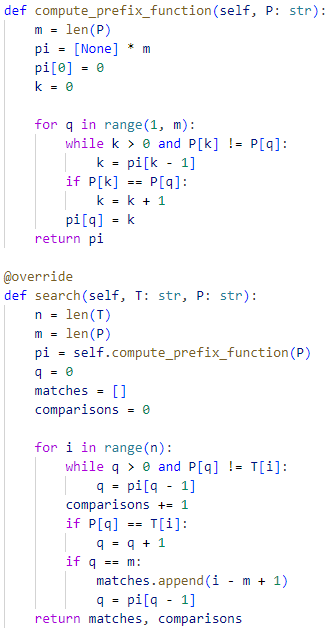
\includegraphics[width=0.4\textwidth]{img/KMP_search.png}
              \caption{Implementazione Python dell'algoritmo KMP}
              \label{fig:KMP-implementation}
          \end{figure}
    \item Motivazioni per l'uso dell'algoritmo KMP:
          \begin{itemize}
              \item Evita confronti ridondanti
              \item Ha stabilità nei casi peggiori
              \item Ottimo in casi di pattern con ripetizioni
              \item Indipendente dalla distribuzione dei caratteri nel testo
              \item La funzione dei prefissi è riutilizzabile per lo stesso pattern su testi diversi
          \end{itemize}
\end{itemize}

\subsection{Assunti ed ipotesi}
Analizziamo adesso gli algoritmi di string matching ``\textbf{ingenuo}'' e \textbf{KMP} dal punto di vista della complessità: entrambi riescono a trovare tutte le occorrenze di un pattern all'interno di un testo ma a causa dei diversi approcci le relative complessità differiscono notevolmente tra loro. In particolare ci concentriamo sull'osservare il numero di confronti e il tempo di esecuzione.
\begin{itemize}
    \item \textbf{Algoritmo ``ingenuo''}: confronta il pattern con ogni possibile sottostringa nel testo. Ciò comporta, nel caso peggiore, un numero di confronti pari a $O((n - m + 1) \cdot m)$, dove \textit{n} è la lunghezza del testo e \textit{m} è la lunghezza del pattern. Tuttavia in alcuni casi quali pattern breve o assenza di occorrenze l'algoritmo può risultare veloce.
    \item \textbf{Algoritmo KMP}: utilizza la funzione dei prefissi per evitare confronti ridondanti. La complessità temporale dell'algoritmo nel caso medio e nel peggiore è $\Theta(n + m)$, cioè una complessità \textbf{lineare}, dove \textit{n} è la lunghezza del testo e \textit{m} è la lunghezza del pattern. Questo lo rende molto più efficiente rispetto all'algoritmo ``ingenuo'' in casi di pattern ripetitivi o con molte occorrenze nel testo.
\end{itemize}
I test verranno effettuati su più scenari andando a variare la lunghezza del testo e del pattern, la densità delle occorrenze e la composizione stessa del pattern e del testo.
\newpage
\noindent Di seguito è rappresentata la tabella riassuntiva delle complessità degli algoritmi analizzati:
\begin{figure}[H]
    \begin{table}[H]
        \centering
        \begin{tabular}{>{\raggedright\arraybackslash}p{2cm}ccc}
            Algoritmo & Tempo di Preprocessing & Tempo di Matching        & Complessità totale       \\
            \midrule
            Ingenuo   & 0                      & $O((n - m + 1) \cdot m)$ & $O((n - m + 1) \cdot m)$ \\
            KMP       & $\Theta(m)$            & $\Theta(n)$              & $\Theta(n + m)$          \\
        \end{tabular}
    \end{table}
    \caption{Tabella delle complessità degli algoritmi analizzati}
    \label{tab:complexity-table}
\end{figure}

\newpage
\section{Documentazione del codice}
\subsection{Schema del contenuto e interazione tra i moduli}
Per svolgere i nostri esperimenti ho, prima di tutto, scritto il codice degli algoritmi a cui faremo riferimento. In questo caso le classi hanno nome \textbf{NaiveMatcher} per l'algoritmo ``ingenuo'' e \textbf{KMPMatcher} per quello KMP. La classe \textbf{StringMatcher} è una classe astratta da cui ereditano le due classi precedenti, attraverso questa posso chiamare il metodo \textbf{\textit{search}} per effettuare la ricerca del pattern all'interno del testo.\\
Ho inoltre implementato la classe \textbf{MatcherTestRunner} che si occupa di chiamare gli algoritmi passando i giusti dati, tenere conto del tempo impiegato e salvare i risultati. Nello stesso pacchetto di quest'ultima classe ho implementato anche la funzione \textbf{\textit{generate\_custom\_graphs}} che va a effetturare gli effettivi test richiamando la classe \textbf{MatcherTestRunner} e genera i relativi grafici.
\begin{figure}[H]
    \centering
    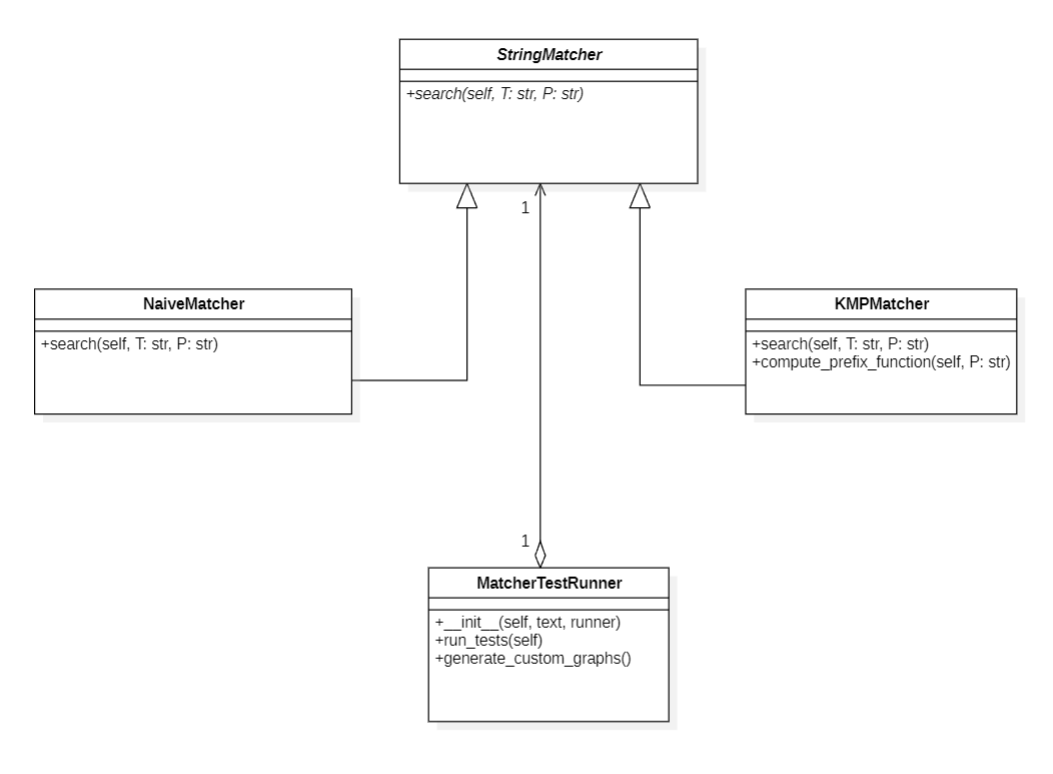
\includegraphics[width=1\textwidth]{img/UML.png}
    \caption{Diagramma delle classi}
    \label{fig:uml-diagram}
\end{figure}

\subsection{Descrizione dei metodi implementati}
In questa parte descriverò le funzionalità di ogni metodo delle classi di cui finora abbiamo parlato.
\begin{itemize}
    \item \textbf{StringMatcher}:
    \begin{itemize}
        \item \textbf{search(self, T: str, P: str)}: Questo metodo è astratto e fa parte di una classe a sua volta astratta. Definisce in questo modo l'interfaccia comune per tutti gli algoritmi di string matching. Ogni algoritmo specifico dovrà implementare questo metodo per eseguire la ricerca del pattern nel testo.\\
        Attraverso questa astrazione il codice diventa più modulare e permette di aggiungere facilmente nuovi algoritmi senza necessità di ulteriori modifiche.
    \end{itemize}
    \item \textbf{NaiveMatcher}
    \begin{itemize}
        \item \textbf{search(self, T: str, P: str)}: Questo metodo effettua l'override del metodo \textbf{search} della classe astratta \textbf{StringMatcher}.\\
        Implementa l'algoritmo di confronto stringhe ``ingenuo''. Scorre il testo posizione per posizione e confronta carattere per carattere con il pattern.
        Restituisce una lista delle posizioni in cui il pattern viene trovato all'interno del testo e il numero totale di confronti effettuati.
        La complessità nel caso peggiore è $O((n - m + 1) \cdot m)$, dove n è la lunghezza del testo e m la lunghezza del pattern.
    \end{itemize}
    \item \textbf{KMPMatcher}
    \begin{itemize}
        \item \textbf{compute\_prefix\_function(self, P: str)}: È un metodo ausiliario che calcola la funzione dei prefissi per il pattern. $\pi[q]$ è un array ausiliario che per ogni posizione del pattern memorizza la lunghezza del più lungo prefisso del pattern che è anche un suffisso della sottostringa P[1...\textit{q}]. Ciò consente all'algoritmo di evitare confronti ridondanti durante la ricerca.
        \item \textbf{search(self, T: str, P: str)}: Questo metodo effettua l'override del metodo \textbf{search} della classe astratta \textbf{StringMatcher}.\\
        Implementa l'algoritmo Knuth-Morris-Pratt per il confronto tra stringhe. Utilizza l'array $\pi[q]$ per determinare in maniera efficiente come muoversi all'interno del testo durante la ricerca del pattern evitando ripetizioni.
        Restituisce le posizioni in cui il pattern è presente nel testo e il numero di confronti effettuati.
        La complessità temporale è $\Theta(n + m)$ , più efficiente dell'approccio ``ingenuo'' specialmente per pattern lunghi o testi ripetitivi.
    \end{itemize}
    \item \textbf{MatcherTestRunner}
    \begin{itemize}
        \item \textbf{\_\_init\_\_(self, text, pattern)}:inizializza l'istanza con il testo e il pattern da cercare e prepara gli oggetti per gli algoritmi di string matching.
        \item \textbf{run\_test(self)}: È il metodo principale che esegue il test di string matching. Chiama i metodi \textbf{search} degli oggetti \textbf{NaiveMatcher} passando il testo e il pattern. Registra quindi il tempo impiegato per ciascun algoritmo, il numero di confronti effettuati e il numero di occorrenze trovate. Restituisce un dizionario con i risultati per entrambi gli algoritmi da utilizzare per la generazione dei grafici.
        \item \textbf{generate\_custom\_graphs()}: Questo metodo genera i grafici per visualizzare i risultati dei test. Al suo interno sono contenuti gli effettivi test da eseguire che vanno a definire il testo e il pattern da utilizzare nella ricerca. Chiama quindi per ogni test il metodo \textbf{run\_test}. Inoltre ogni caso ha al suo interno due cicli for: uno necessario per variare le dimensioni del test o del pattern in modo da ottenere un grafico più completo, l'altro per fare una media dei risultati ottenuti in modo da eliminare dal grafico finale eventuali picchi dovuti al fatto che i tempi di ricerca sono molto piccoli.
    \end{itemize}
\end{itemize}

\newpage

\section{Descrizione degli esperimenti condotti e analisi dei risultati sperimentali}
\subsection{Dati utilizzati}
Per effettuare una valutazione sperimentale delle prestazioni degli algoritmi analizzati sono stati progettati otto casi di test, ognuno mirato a studiare uno specifico aspetto dell'efficienza e del comportamento degli algoritmi.\\
I dati sono stati generati in modo pianificato per garantire che ogni test generasse un grafico utile e significativo.\\
Di seguito vediamo i vari test effettuati:
\begin{enumerate}
    \item \textbf{Tempo vs lunghezza testo}: Misura l'andamento temporale al crescere della dimensione del testo.
    \item \textbf{Confronti vs lunghezza testo}: Valuta il numero di confronti effettuati al variare della lunghezza del testo.
    \item \textbf{Caso peggiore}: Calcola il numero di confronti nel caso peggiore (pattern quasi uguale al testo).
    \item \textbf{Sovrapposizioni del pattern}: Guarda il numero di confronti con match sovrapposti.
    \item \textbf{Tempo vs lunghezza pattern}: Misura l'andamento temporale al crescere della dimensione del pattern.
    \item \textbf{Confronti vs densità di match}: Analizza il comportamento in testi misti.
    \item \textbf{Testi casuali vs testi ripetitivi}: Confronta l'efficienza degli algoritmi nei casi di testi casuali e di quelli ripetitivi.
    \item \textbf{Tempo di preprocessing KMP}: Analizza il tempo di preprocessing dell'algoritmo KMP al variare della lunghezza del pattern.
\end{enumerate}
In particolare notiamo come nei casi 1, 2 e 3 vengono usati testi creati come concatenazioni ripetute di una stringa base e pattern fissi.\\
Nel test 3, il caso peggiore, il pattern è stato creato in modo tale da essere quasi uguale al testo, differisce in un solo carattere alla fine, andando a obbligare l'algoritmo ``ingenuo'' aripetere quasi tutti i confronti fino alla fine del testo.\\
Il caso 4 utilizza pattern sovrappposti che evidenziano la capacità dell'algoritmo KMP di evitare confronti ridondanti.\\
Il test 7 confronta l'efficienza su un testo completamente casuale e uno totalmente ripetitivo, mostrando in questo modo i casi favorevoli e sfavorevoli per entrambi gli algoritmi.\\
Il caso 8 infine mostra in modo isolato il tempo di calcolo della funzione dei prefissi dell'algoritmo KMP al variare della lunghezza del pattern.\\

\subsection{Misurazioni}
Le misurazioni dei tempi di eleborazione degli algoritmi sono state effettuate nel metodo \textbf{run\_test} della classe \textbf{MatcherTestRunner}. Per poterle eseguire è stato utilizzato il modulo \textbf{time} importato all'inizio del file \textit{string\_matcher\_runner.py}.\\
Vediamo adesso nel dettaglio come è stata effettuata la misurazione del tempo:
\begin{figure}[H]
    \centering
    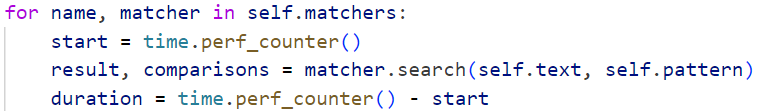
\includegraphics[width=0.8\textwidth]{img/Tempo.png}
    \caption{Misurazione del tempo}
    \label{fig:time-measurement}
\end{figure}
\begin{enumerate}
    \item \textbf{Ciclo for}: necessario a scorrere tra tutti gli algoritmi di string matching implementati nel progetto per poter poi fare le misurazioni e poter stampare i relativi risultati.
    \item \textbf{Inizializzazione}: attraverso l'utilizzo del modulo \textbf{time} viene inizializzato il tempo di inizio della misurazione e salvato nella variabile \textit{start}.
    \item \textbf{Chiamata degli algoritmi}: viene chiamato il metodo \textbf{search} degli string matcher implementati, passando il testo e il pattern da cercare. Gli output vegono poi salvati nelle variabili \textit{result} e \textit{comparisons}.
    \item \textbf{Fine misurazione}: viene poi calcolato il tempo di esecuzione sottraendo il tempo di inizio salvato nella variabile \textit{start} dal tempo attuale. Il risultato viene poi salvato nella variabile \textit{duration}.
\end{enumerate}
Nella seguente figura è riportata l'implementazione di uno dei test per poter descrivere la struttura del codice:
\begin{figure}[H]
    \centering
    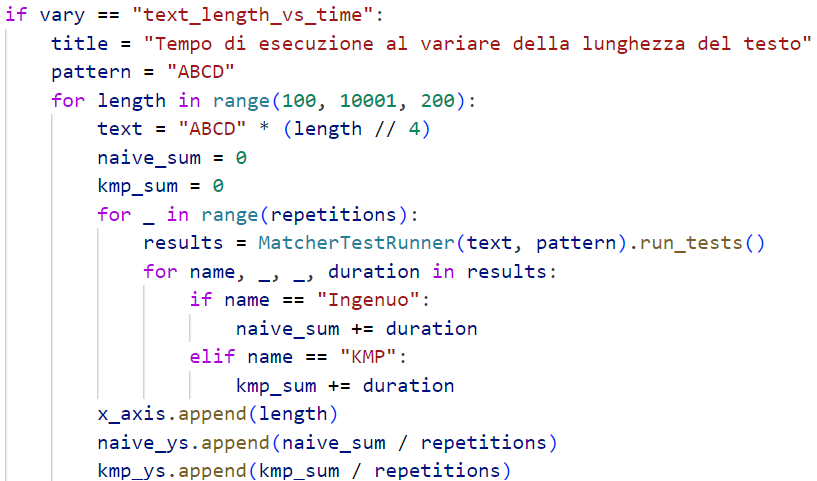
\includegraphics[width=0.8\textwidth]{img/Test.png}
    \caption{Implementazione di uno dei test}
    \label{fig:test-implementation}
\end{figure}
\begin{enumerate}
    \item Il test inizia con un if che va a controllare quale caso di test si sta eseguendo.
    \item Successivamente è riportato il titolo del test che andrà ad apparire in alto nel grafico.
    \item Viene ora definito il pattern che sarà ricercato nel testo definito nelle successive righe.
    \item Il for è necessario per variare la lunghezza del testo stesso in modo da poter generare in questo modo il grafico.
    \item Viene di seguito quindi definito il testo da utilizzare per l'esperimento sfruttando la variabile \textit{length} definita nel for. Notiamo come la lunghezza viene fatta modulo 4, ovvero la lunghezza base del testo, per poter ottenere un testo complessivo la cui lunghezza totale è il più vicino possibile alla variabile \textit{length}.
    \item Sono poi definite le variabili somma per i relativi algoritmi necessarie poi per poter fare la media dei risultati. Quindi viene fatto un ciclo for che ripete il test per un numero di volte pari alla variabile \textit{repetitions} grazie al quale vengono rimossi dal grafico eventuali picchi anomali dovuti alla ricerca del pattern molto veloce.
    \item Adesso viene fatto l'effettivo test andando a chiamare il metodo \textbf{run\_tests} passando dunque il pattern e il testo sopra definiti.
    \item In questo for vengono salvati nelle relative variabili somma i risultati (in questo caso i tempi) di un singolo test.
    \item Infine viene impostata nelle ascisse una variabile da analizzare (la lunghezza del testo in questo caso) e nelle ordinate la media dei risultati dei vari test (media dei tempi per questo test), sia per l'algoritmo ``ingenuo'' che per il KMP per poter così visualizzare il confronto sullo stesso grafico.
\end{enumerate}
Infine riporto l'implementazione della parte di codice necessaria a generare i grafici:
\begin{figure}[H]
    \centering
    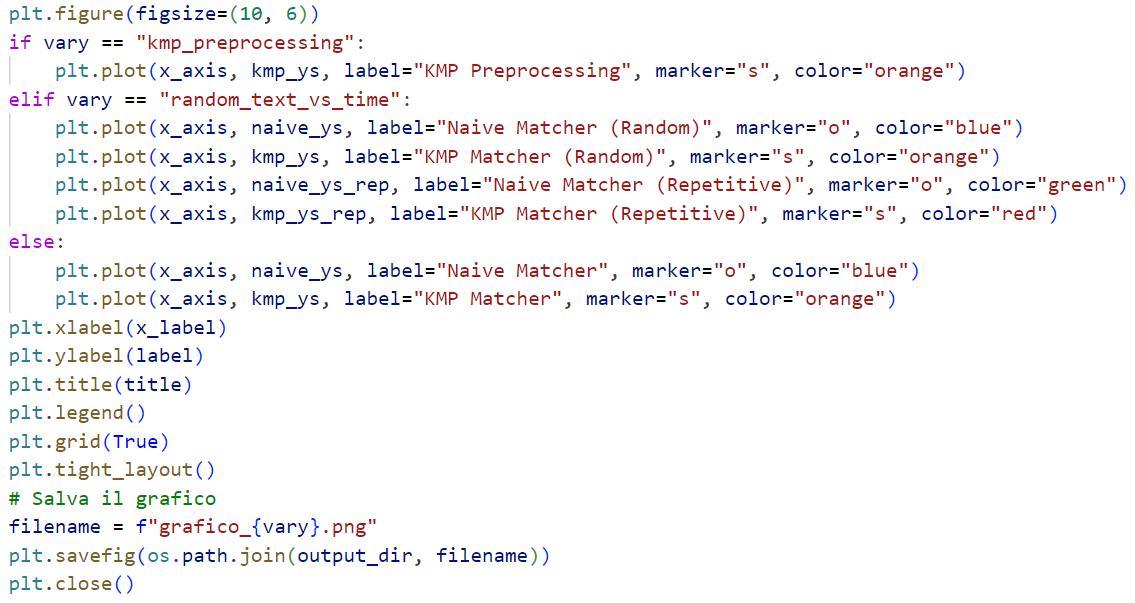
\includegraphics[width=1\textwidth]{img/Plot_graphs.png}
    \caption{Implementazione delle operazioni per creare i grafici}
    \label{fig:plot-graphs}
\end{figure}
\noindent Da notare come sono presenti due if per poter, nel primo, generare un grafico con visualizzato solamente l'algoritmo KMP mentre, nel secondo, poter visualizzare tutti e quattro i risultati del relativo test anziché i classici due.

\newpage
\subsection{Risultati sperimentali e commenti analitici}
In questo paragrafo andremo ad analizzare più nel dettaglio i singoli test e a visualizzare e commentare i relativi grafici.
\begin{itemize}
    \item \textbf{Tempo di esecuzione al variare della lunghezza del testo}\\
        In questo test osserviamo il tempo di esecuzione al variare della lunghezza del testo. Il pattern è fissato mentre il testo aumenta in lunghezza. Dal grafico in figura \ref{fig:test-1} possiamo notare come l'algoritmo KMP abbia una crescita più lineare rispetto all'algoritmo ``ingenuo''. Inoltre notiamo anche il fatto che all'aumentare della lunghezza del testo l'algoritmo KMP è più veloce dell'algoritmo ``ingenuo'' nel trovare le occorrenze del pattern.
        \begin{figure}[H]
            \centering
            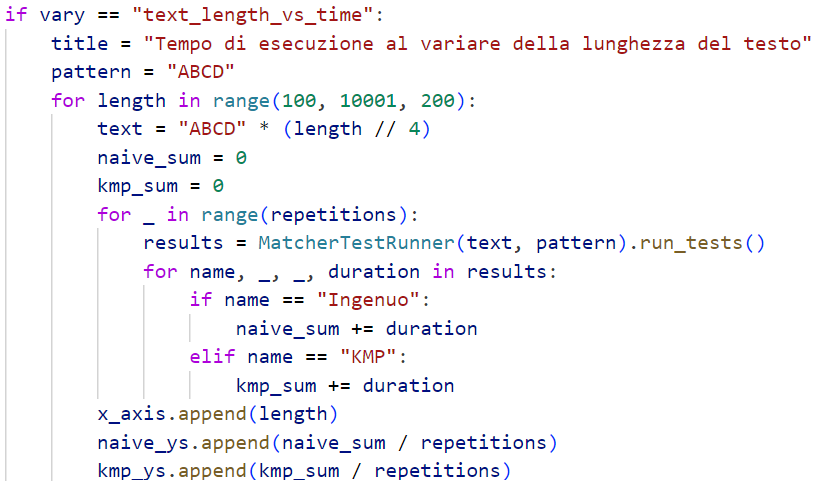
\includegraphics[width=0.8\textwidth]{img/Test1.png}
            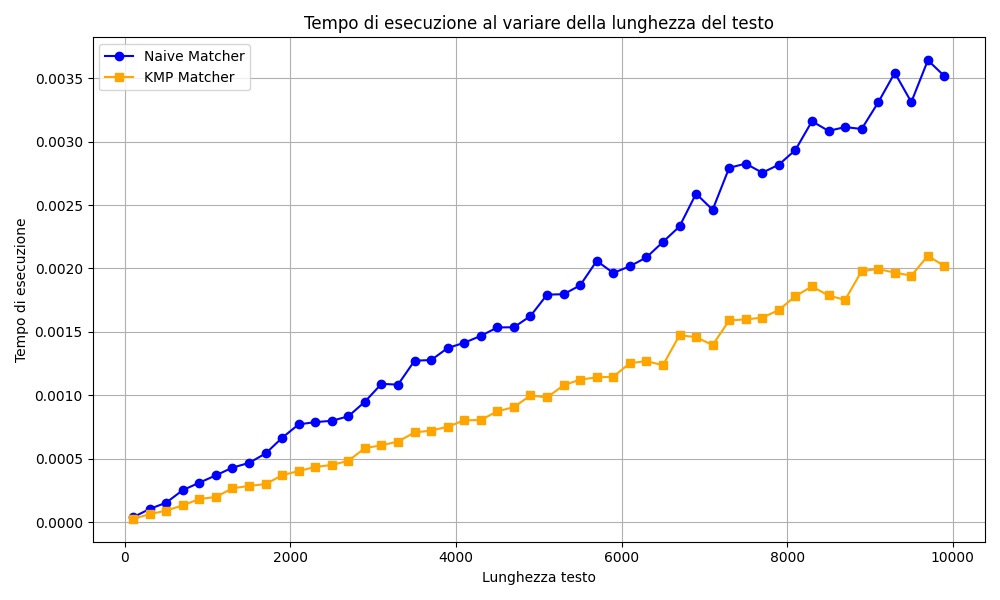
\includegraphics[width=0.8\textwidth]{img/Graph1.png}
            \caption{Tempo di esecuzione al variare della lunghezza del testo}
            \label{fig:test-1}
        \end{figure}
    \newpage
    \item \textbf{Numero di confronti al variare della lunghezza del testo}\\
        In questo test osserviamo il numero di confronti effettuati al variare della lunghezza del testo. Il pattern è fissato mentre il testo aumenta in lunghezza. Dal grafico in figura \ref{fig:test-2} possiamo notare come l'algoritmo KMP abbia la capacità di evitare confronti ridondanti risultando in una crescita più lenta rispetto all'algoritmo ``ingenuo'' che cresce più rapidamente, ovvero effettua più confronti per torvare tutte le occorrenze del pattern.
        \begin{figure}[H]
            \centering
            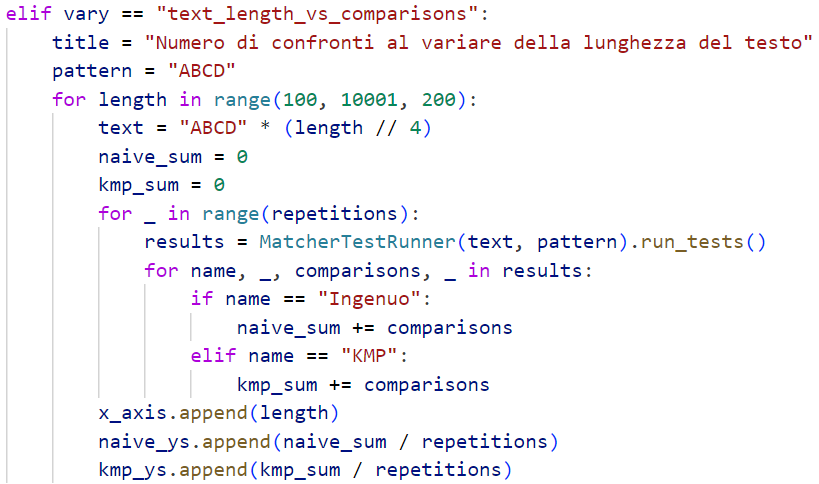
\includegraphics[width=0.8\textwidth]{img/Test2.png}
            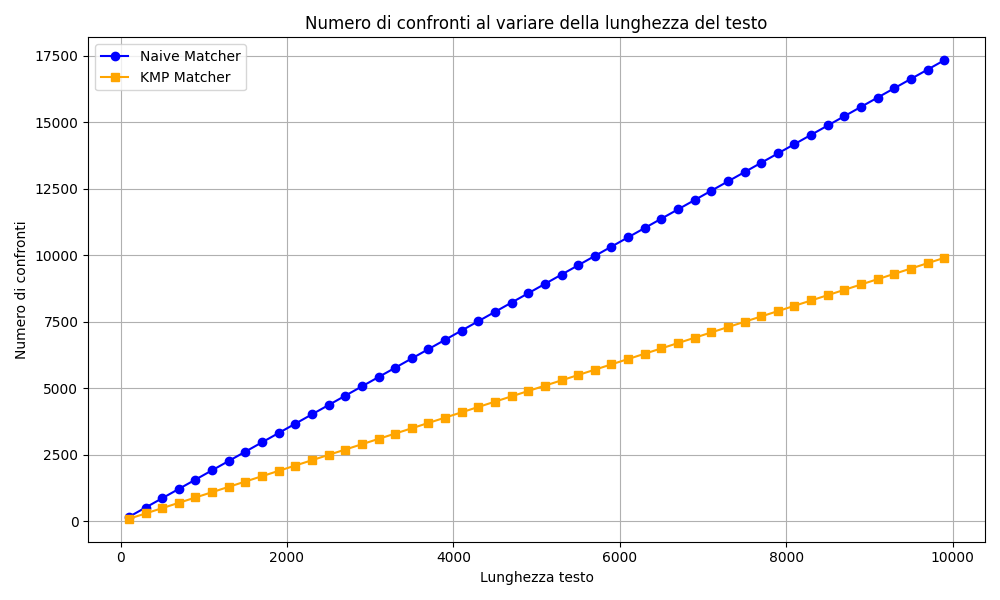
\includegraphics[width=0.8\textwidth]{img/Graph2.png}
            \caption{Numero di confronti al variare della lunghezza del testo}
            \label{fig:test-2}
        \end{figure}
    \newpage
    \item \textbf{Numero di confronti nel caso peggiore (pattern quasi uguale al testo)}\\
        In questo test osserviamo il numero di confronti effettuati nel caso peggiore, ovvero quando il pattern è quasi uguale al testo. In questo caso sia il pattern che il testo aumentano in lunghezza. Dal grafico in figura \ref{fig:test-3} possiamo notare come l'algoritmo ``ingenuo'' abbia una crescita esponenziale rispetto all'algoritmo KMP che rimane lineare. Ciò è nuovamente dovuto alla capacità dell'algoritmo KMP di evitare confronti ridondanti, mentre l'algoritmo ``ingenuo'' è costretto a confrontare ogni carattere del pattern con ogni carattere del testo.
        \begin{figure}[H]
            \centering
            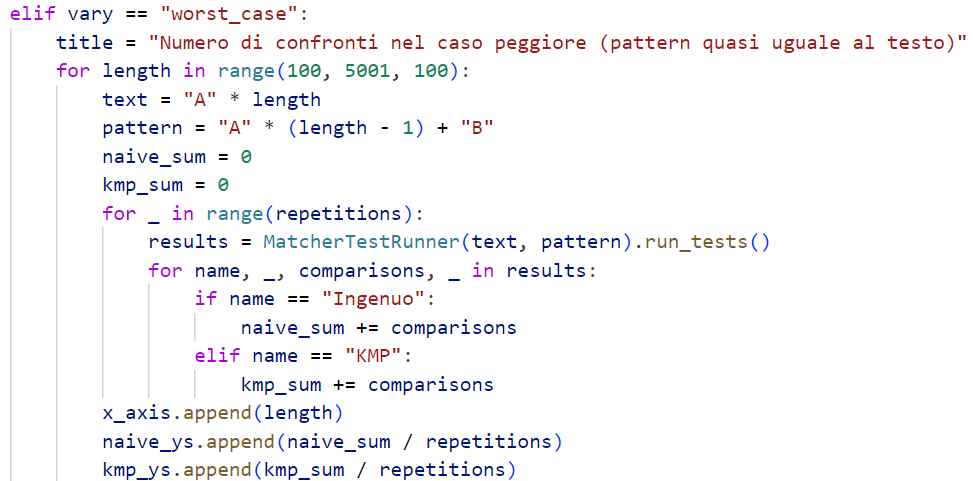
\includegraphics[width=0.8\textwidth]{img/Test3.png}
            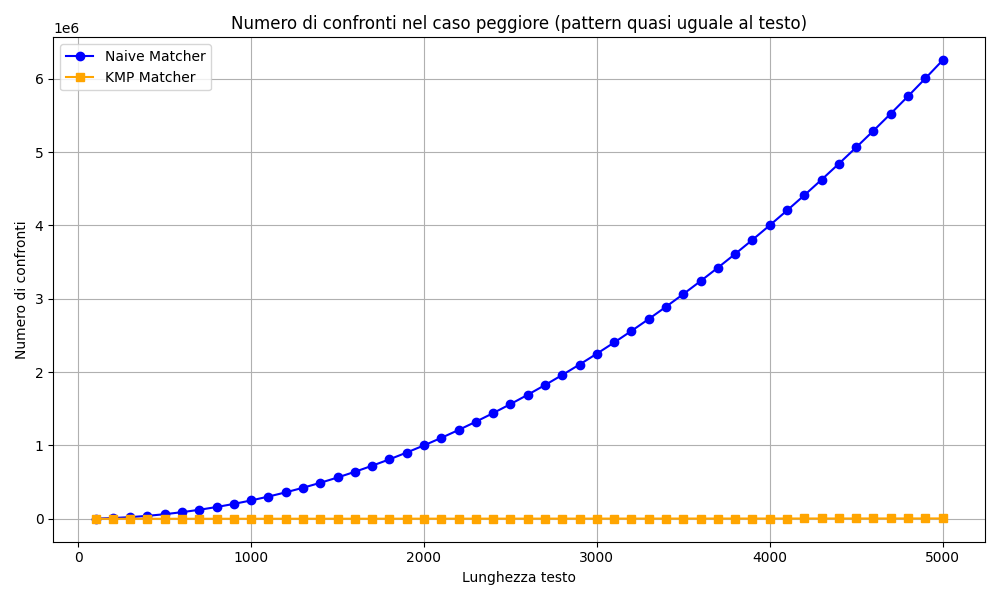
\includegraphics[width=0.8\textwidth]{img/Graph3.png}
            \caption{Numero di confronti nel caso peggiore (pattern quasi uguale al testo)}
            \label{fig:test-3}
        \end{figure}
    \newpage
    \item \textbf{Numero di confronti con match sovrapposti}\\
        In questo test osserviamo il numero di confronti effettuati con match sovrapposti. In questo caso il pattern rimane costante mentre il testo aumenta in lunghezza. Dal grafico in figura \ref{fig:test-4} notiamo nuovamente che l'algoritmo KMP ha una crescita più lenta rispetto all'algoritmo ``ingenuo''. In questo caso KMP è molto più efficiente andando a evitare controlli già effettuati.
        \begin{figure}[H]
            \centering
            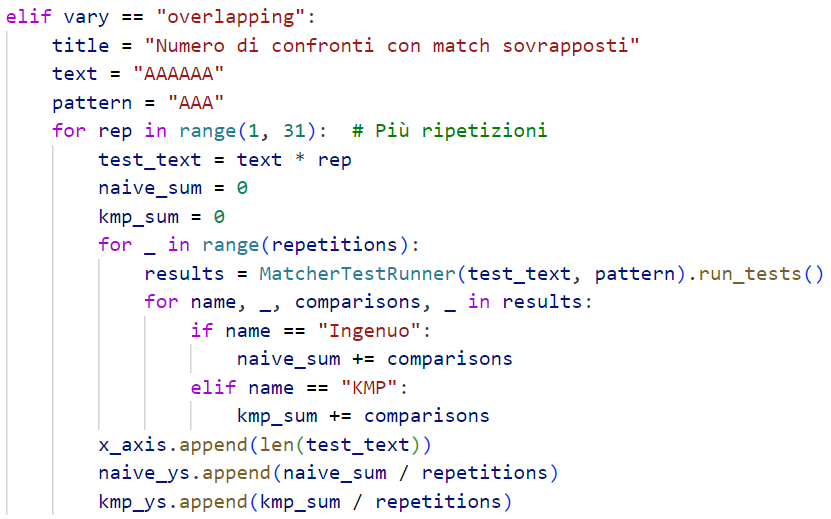
\includegraphics[width=0.8\textwidth]{img/Test4.png}
            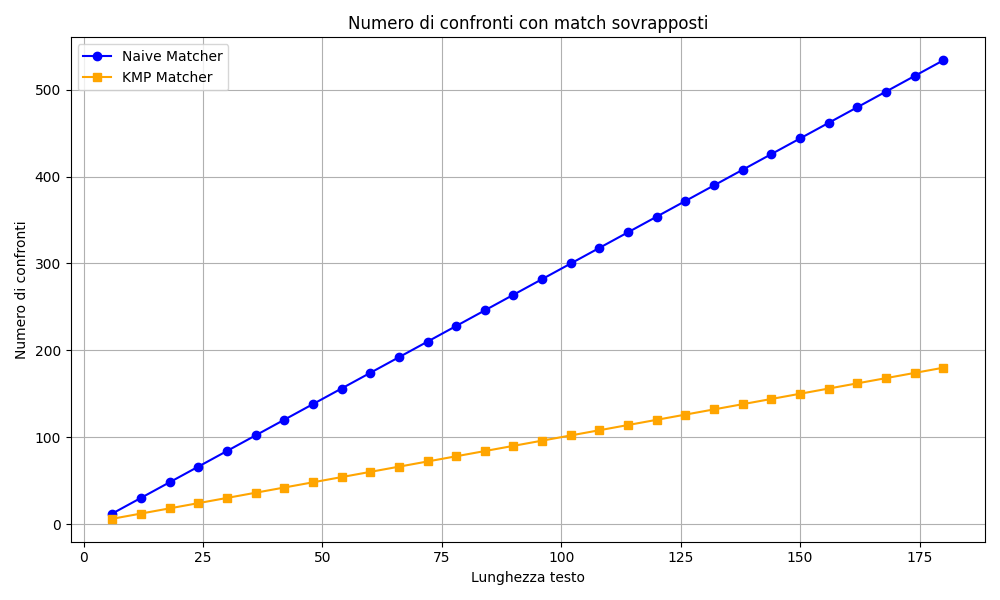
\includegraphics[width=0.8\textwidth]{img/Graph4.png}
            \caption{Numero di confronti con match sovrapposti}
            \label{fig:test-4}
        \end{figure}
    \newpage
    \item \textbf{Tempo di esecuzione al variare della lunghezza del pattern}\\
        In questo test osserviamo il tempo di esecuzione al variare della lunghezza del pattern. In questo caso il pattern aumenta in lunghezza mentre il testo rimane costante. Dal grafico in figura \ref{fig:test-5} vediamo che l'aumentare della lunghezza del pattern comporta un aumento del tempo di esecuzione notevole per l'algoritmo ``ingenuo'' a differenza del KMP che in confronto ha una crescita quasi impercettibile. 
        \begin{figure}[H]
            \centering
            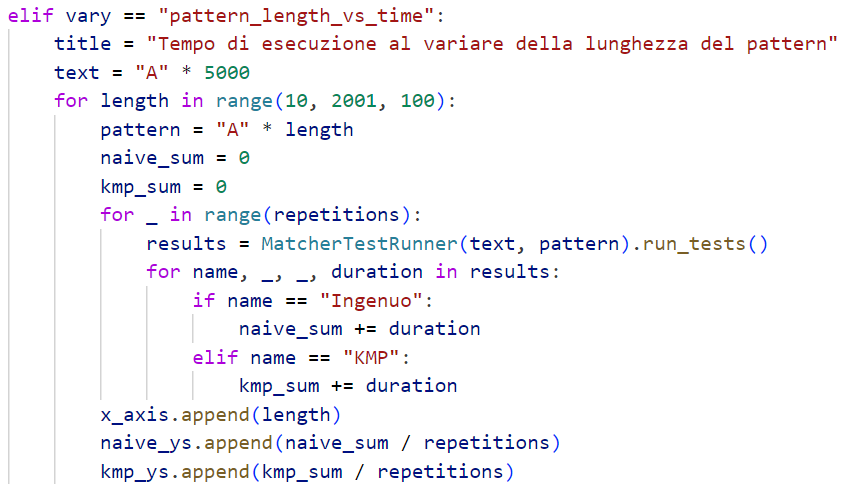
\includegraphics[width=0.8\textwidth]{img/Test5.png}
            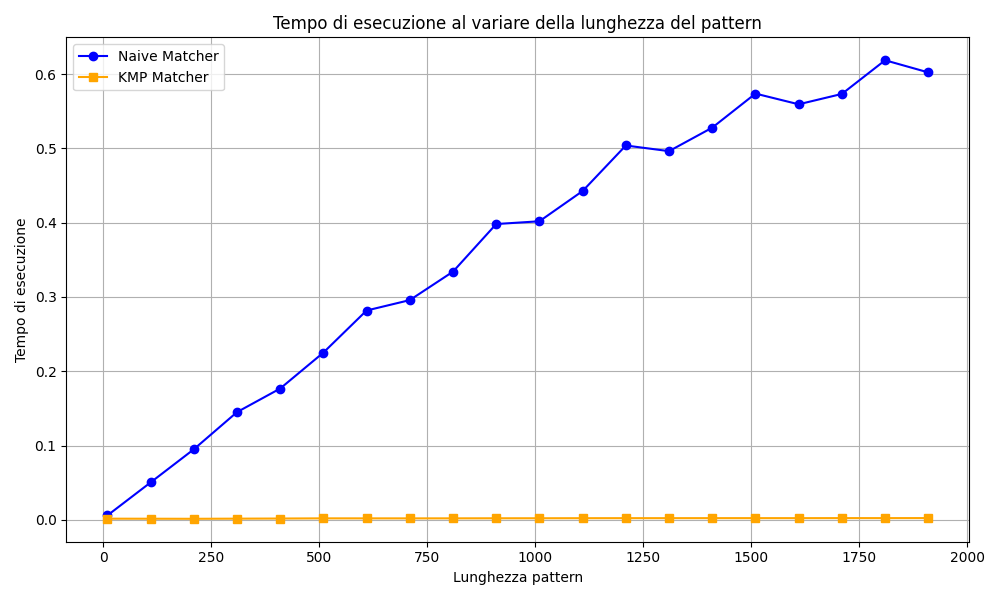
\includegraphics[width=0.8\textwidth]{img/Graph5.png}
            \caption{Tempo di esecuzione al variare della lunghezza del pattern}
            \label{fig:test-5}
        \end{figure}
    \newpage
    \item \textbf{Numero di confronti in funzione della densità di match}\\
        In questo test osserviamo come la frequenza di occorrenze del pattern nel testo influisca sull'efficienza. In questo caso il pattern rimane costante mentre il testo viene calcolato sulla base della densità di occorrenze. Dal grafico in figura \ref{fig:test-6} osserviamo che per bassa densità di occorrenze entrambi gli algoritmi facciano molti confronti mentre all'aumentare della densità l'algoritmo KMP riesca a diminuire più rapidamente il numero di confronti.
        \begin{figure}[H]
            \centering
            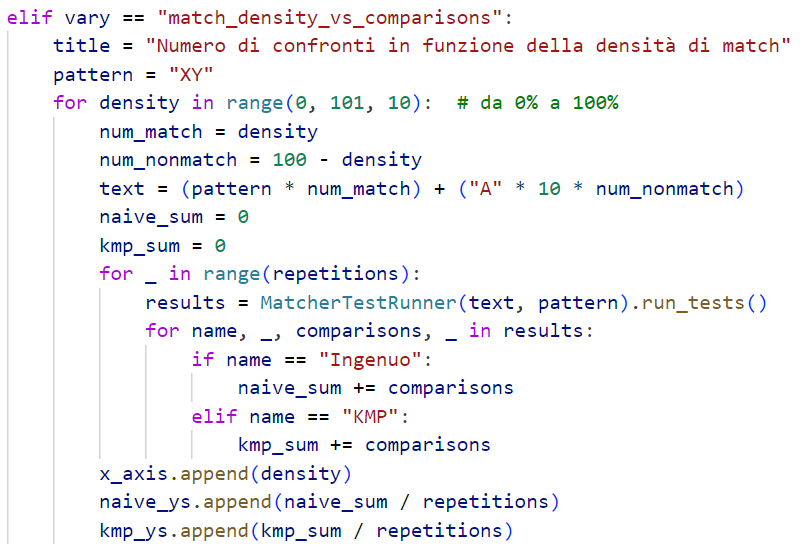
\includegraphics[width=0.8\textwidth]{img/Test6.png}
            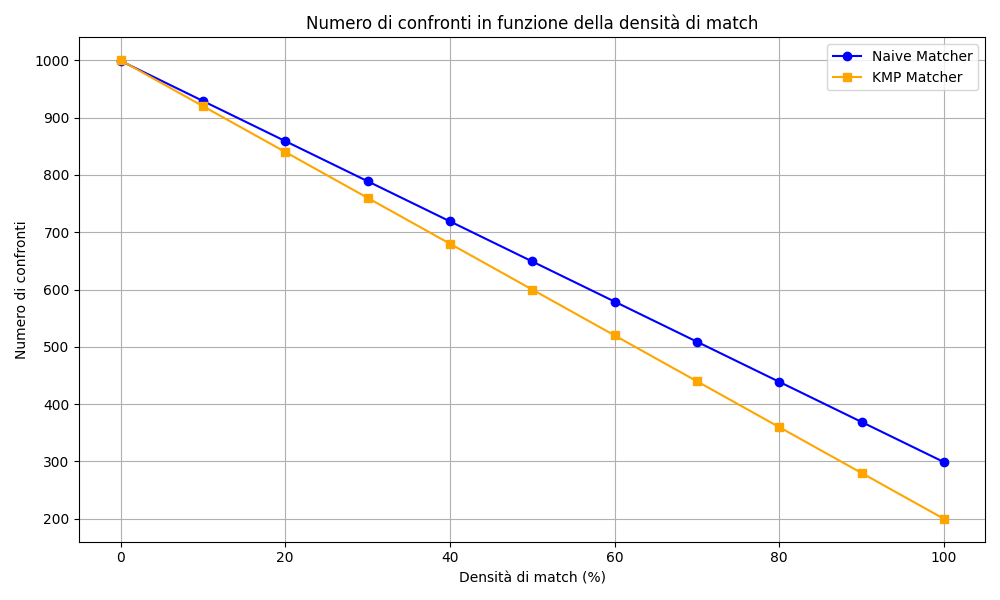
\includegraphics[width=0.8\textwidth]{img/Graph6.png}
            \caption{Numero di confronti in funzione della densità di match}
            \label{fig:test-6}
        \end{figure}
    \newpage
    \item \textbf{Tempo di esecuzione su testo casuale e ripetitivo}\\
        In questo test analizziamo il tempo di esecuzione sia su un testo totalmente casuale che su uno ripetitivo. In questo caso il pattern rimane costante mentre, una volta, il testo è calcolato in modo randomico, nell'altra viene ripetuto per una certa lunghezza. Dal grafico in figura \ref{fig:test-7}, in cui sono riportati i grafici per i quattro casi, notiamo come l'algoritmo KMP riesca a mantenere un tempo di esecuzione molto più basso in entrambi i casi.
        \begin{figure}[H]
            \centering
            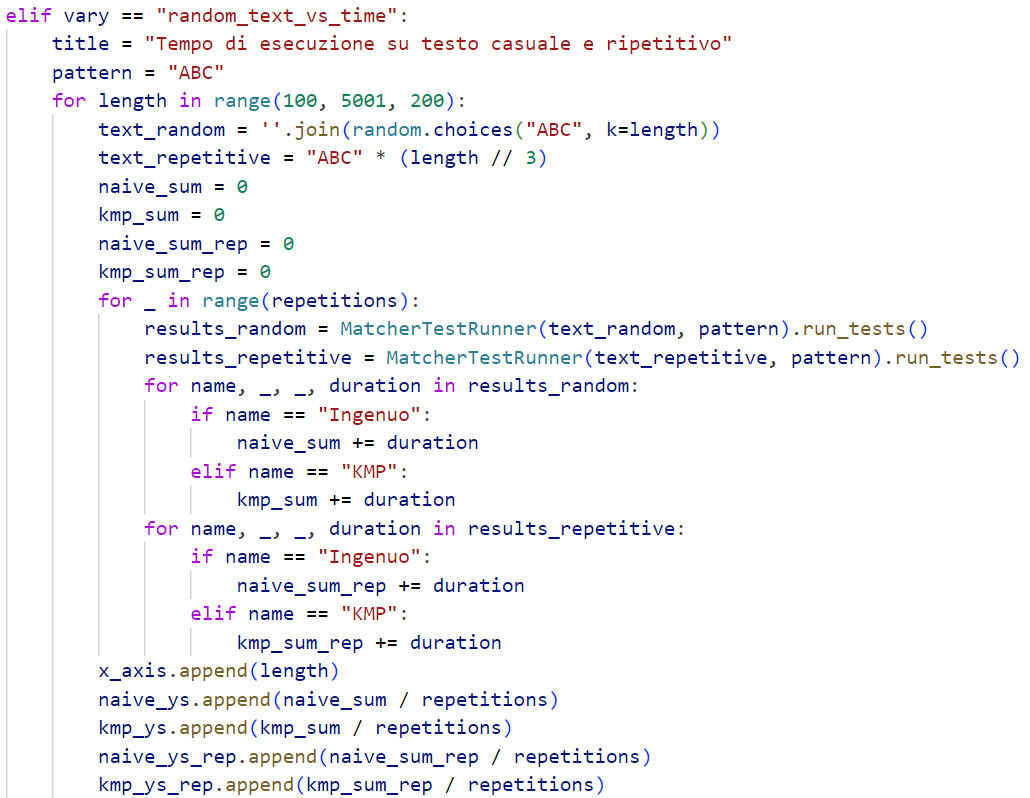
\includegraphics[width=0.8\textwidth]{img/Test7.png}
            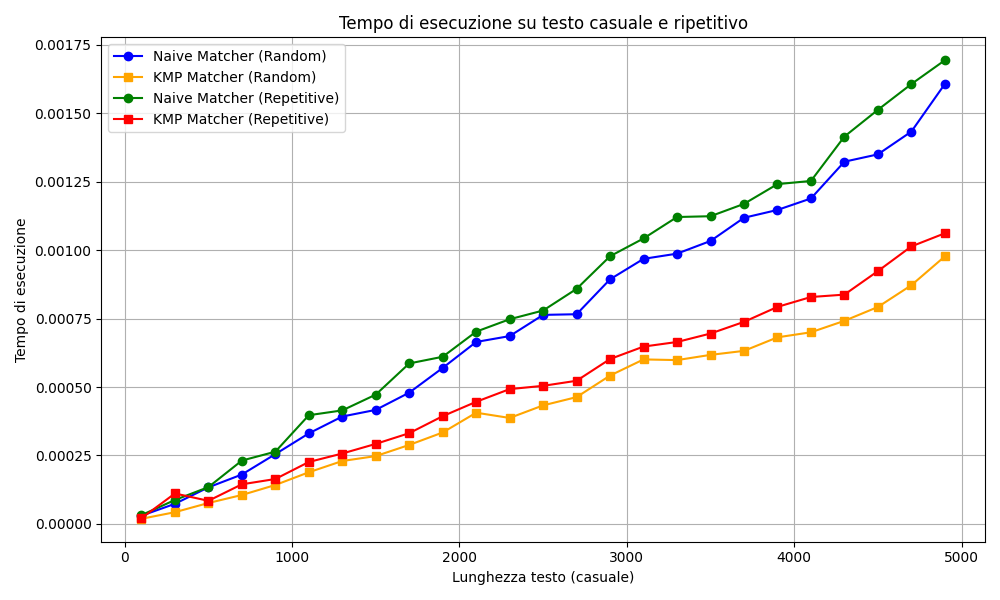
\includegraphics[width=0.8\textwidth]{img/Graph7.png}
            \caption{Tempo di esecuzione su testo casuale e ripetitivo}
            \label{fig:test-7}
        \end{figure}
    \newpage
    \item \textbf{Tempo di preprocessing KMP al variare della lunghezza del pattern}\\
        In questo ultimo test studiamo il tempo di preprocessing dell'algoritmo KMP al variare della lunghezza del pattern. Vediamo quindi come il pattern aumenti in lunghezza. Dal grafico in figura \ref{fig:test-8}, in cui è ovviamente riportato solo la parte dell'algoritmo KMP, notiamo come il tempo di preprocessing cresca approssimativamente in modo lineare, ciò è dovuto al costo anch'esso lineare della funzione dei prefissi. Il rumore presente nel grafico è dovuto ai tempi molto piccoli di esecuzione.
        \begin{figure}[H]
            \centering
            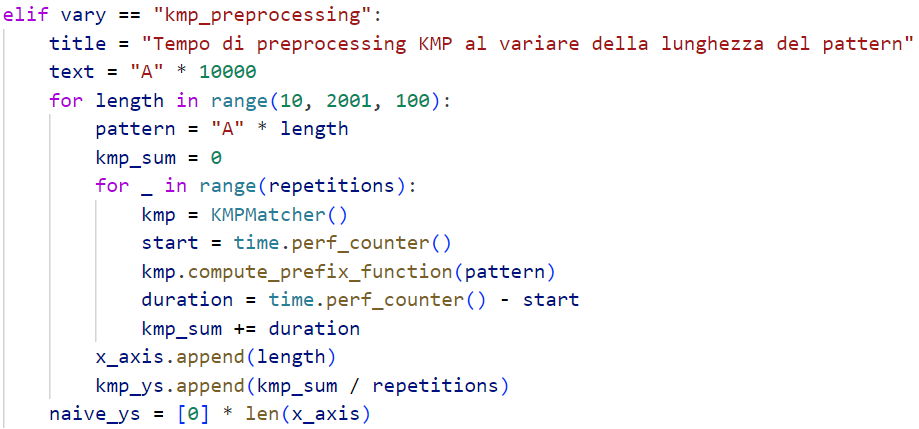
\includegraphics[width=0.8\textwidth]{img/Test8.png}
            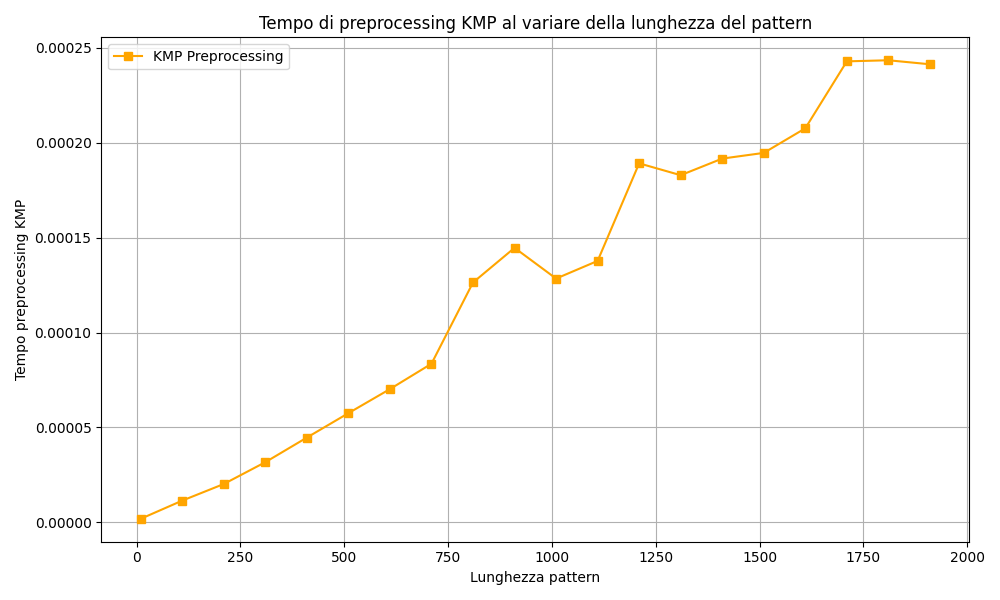
\includegraphics[width=0.8\textwidth]{img/Graph8.png}
            \caption{Tempo di preprocessing KMP al variare della lunghezza del pattern}
            \label{fig:test-8}
        \end{figure}
\end{itemize}

\newpage
\subsection{Tesi e sintesi finale}
A seguito dei nostri risultati e analisi nella sezione 4.3, possiamo trarre le seguenti conclusioni:
\begin{itemize}
    \item Nei test su testi di grandi dimensioni e pattern lunghi o ripetitivi, l'algoritmo Knuth-Morris-Pratt ha dimostrato un costo lineare $\Theta(n + m)$ sia in termini di tempo che di confronti.\\
    L'algoritmo Naïve, al contrario, cresce quadraticamente nel worst-case $O((n - m + 1) \cdot m)$, rendendosi rapidamente non praticabile al crescere di \textit{n} o \textit{m}.
    \item Con pattern quasi identico al testo (test worst-case), l'algoritmo ``ingenuo'' ha effettuato un numero di confronti prossimo a \textit{$n \cdot m$} generando un grafico esponenziale mentre KMP ha mantenuto un andamento lineare, confermando la robustezza della funzione dei prefissi nel ridurre i confronti ridondanti.
    \item Nei testi con molti match sovrapposti, l'algoritmo ``ingenuo'' ha ripetuto numerose volte gli stessi controlli, mentre KMP ha sfruttato le informazioni già calcolate, riducendo drasticamente i confronti ridondanti.
    \item Il tempo di esecuzione del Naïve aumenta sensibilmente all'aumentare di \textit{m}, mentre KMP rimane quasi piatto: il pattern più lungo incide su KMP solo nella fase di preprocessing $O(m)$, trascurabile in confronto alla fase di matching $O(n)$.
    \item Con densità di match variabile o con testi casuali e ripetitivi, KMP ha mostrato prestazioni migliori e più stabili. L'algoritmo ``ingenuo'' ha invece performato su testi casuali con pochi match.
\end{itemize}
In conclusione, gli esperimenti effettuati confermano le previsioni teoriche: KMP offre prestazioni superiori e più prevedibili, mentre l'algoritmo ``ingenuo'' rimane una valida alternativa solo per testi e pattern di piccole dimensioni o in assenza di occorrenze.

\newpage
\addcontentsline{toc}{section}{Riferimenti bibliografici}
\begin{thebibliography}{9}
\bibitem{cormen}
TThomas H. Cormen, Charles E. Leiserson, Ronald L. Rivest, Clifford Stein (2009) Introduzioneagli algoritmi e strutture dati Terza edizione, McGraw Hill.21
\end{thebibliography}

\end{document}